\chapter{Eigenvalue Computation}		\label{Sec:evol_mats}



\section{Introduction}   \label{Subsec:evol_mats-intro}


In this chapter we examine the \textit{evolving matrix eigenvalue problem} (EMEP) in Algorithm \ref{Alg:PGD} and develop a new strategy for solving this problem.


Section \ref{Subsec:evol_mats-spectral_props} defines the EMEP and examines its computational costs and evolving spectrum across matrix iterates $A_k$.  
In particular, we observe that the algebraically largest eigenvalues tend to cluster as the algorithm proceeds, leading to more difficult eigenvalue problems for later matrix iterates.  
To handle these eigenvalue problems, Section \ref{Subsec:evol_mats-IRAM} reviews the \textit{implicitly restarted Arnoldi method} (IRAM) \cite{sorensen1992implicit}, a modern Krylov subspace method. 
The convergence behavior of the IRAM is based on the spectrum of the given eigenvalue problem as well as the IRAM parameters chosen by the user.
To understand and exploit the convergence behavior of the IRAM, Section \ref{Subsec:evol_mats-IRAM} reviews the subroutines of the IRAM and summarizes relevant convergence results.


Next, Section \ref{Subsec:evol_mats-adaptive_IRAM} presents \textit{the IRAM with adaptive parameter selection}, a new strategy for solving the EMEP by adaptively changing
the number of requested eigenvalues $r$ in the IRAM (Algorithm \ref{Alg:IRAM}).
Section \ref{Subsec:evol_mats-correl_btwn_EMEP_and_IRAM} closely examines the EMEP for two PLGD models with Gaussian noise (\ref{Eqn:PhaseLift-GD_Gaussian_noise}) to demonstrate an observed correlation between the clustering of the algebraically largest eigenvalues in the EMEP and an increase in the optimal choice of parameter $r$ in the IRAM.
We see that the IRAM with adaptive parameter selection properly tracks the optimal choice of $r$ for these models.
Performance results for the IRAM with adaptive parameter selection are presented in  Chapter \ref{Sec:Numerics}.
Also note that all \emep \ experiments in this chapter are performed with Algorithm \ref{Alg:PGD} using the new termination conditions (\ref{Eqn:term_crit_new-primal_difference}) and (\ref{Eqn:term_crit_new-dual_difference}) established in Chapter \ref{Sec:PLGD_term_crit} and are available for reproduction.\footnote{\url{https://github.com/Will-Wright/low-rank-opt-rapid-eig}}




\section{The Evolving Matrix Eigenvalue Problem}		\label{Subsec:evol_mats-spectral_props}


In this section we examine the sequence of eigenvalue problems in Algorithm \ref{Alg:PGD}, which we define as the \textit{evolving matrix eigenvalue problem} (EMEP).
We will see that the EMEP is the most computationally expensive subroutine in Algorithm \ref{Alg:PGD}.  
We also observe that the EMEP matrix iterates have a spectrum which evolves in a predictable way from early to later iterates.




\subsection{Definition} 	\label{Subsubsec:evol_mats-EMEP_definition}


We begin by formally defining the EMEP.
Generally speaking, we are concerned with a sequence of eigenvalue problems in which each eigenvalue problem is dependent on the results of the previous problem.  
For each iterate $k$ in this sequence of problems, we have some Hermitian matrix iterate $A_k \in \caH^n$ and seek its $j$ algebraically largest eigenvalues $\Lambda^{(k)}_j$ and the corresponding eigenvectors $V^{(k)}_j$.  
%Next, the previous set of basis matrices $\caV_{k} = \{ V^{(i)}_j \}_{i=0}^{k}$ are used to find the next matrix iterate $A_{k+1}$.  
%More specifically, we are concerned with problems of the form
%\begin{equation} 		\label{Eqn:EMEP_general}
%\begin{array}{ll}
%\textnormal{for}
%	&	k = 1, 2, \ldots, K		\\
%\textnormal{find}	
%	&	\left( \Lambda^{(k)}_j, \ V^{(k)}_j \right) \textnormal{ of } A_k
%\end{array}
%\end{equation}
%where $\Lambda^{(k)}$ are the $j$ algebraically largest eigenvalues of $A_k$, $V_k$ is the matrix of corresponding eigenvectors, $A_k \in \caH^n$ is dependent on $\caV_{k} = \{ V^{(i)}_j \}_{i=0}^{k}$, and $V_0 \in \bbC^{n \times j}$ is an initial basis matrix.
Some examples of this problem include subspace tracking in signal processing (see, e.g., \cite{comon1990tracking}, \cite{stewart1992updating}, \cite{yang1995projection}, \cite{doukopoulos2008fast}), matrix completion (e.g., \cite{ngo2012scaled}), and the Kohn-Sham equation in density functional theory (e.g., \cite{saad2010numerical}).



%To see that each eigenvalue problem in Algorithm \ref{Alg:PGD} is dependent on the results of the previous eigenvalue problems, 

%(Also note that the iterate $k$ does not correspond to the iterate number in Algorithm \ref{Alg:PGD} because step 6 involves a linesearch which may involve more than one eigenvalue problem.)  

%We will show that each matrix iterate $A_k = \caA^*y_k$ in Algorithm \ref{Alg:PGD} is computed using a variable $y_k$ which is dependent on the previous set of basis vectors $\caV_{k-1} = \{ v_1^{(i)} \}_{i=0}^{k-1}$.  

%It can be shown inductively that $y_k$ is a function of $\caV_{k-1}$.  The initial iterate $k = 0$ corresponds to the first eigenvalue problem in Algorithm \ref{Alg:PGD}, where $y_0 = \Pi_\caC(b)$ is initialized using the observation vector $b$ and is independent of any eigenvector.  



To define the EMEP, first note that each eigenvalue problem in Algorithm \ref{Alg:PGD} (steps 2, 6, and 14) requires the two algebraically largest eigenvalues of the matrix iterate $A_k = \caA^*y_k$, where $\caA^*$ is defined as (\ref{Eqn:A_definition_with_masks}).
In Algorithm \ref{Alg:PGD}, the matrix $A_0$ is initialized as $A_0 = \caA^*b$, where $b$ is the observation vector in the PLGD model (\ref{Eqn:PhaseLift-P-GD}).
For each iterate $k >0$, the update matrix $A_k = \caA^*y_k$ is computed with $y_k = \Pi_{\caC}(y_{k-1}- \alpha_{k-1}  g_{k-1})$, where the gradient $g_{k-1} = \caA(v_{k-1} v_{k-1}^*)$ is a function of $v_{k-1}$ and the steplength $\alpha_{k-1}$ is determined using a linesearch on the minimization problem
\begin{equation}			\label{Eqn:EMEP_linesearch_prob_in_evol_mats_chapter}
\begin{array}{ll}
\min\limits_{\substack{\alpha}}
	&	\lambda_1 \left( \caA^* ( \Pi_\caC ( y_{k-1} - \alpha g_{k-1} ) )  \right).
\end{array}
\end{equation}
Thus we define the sequence of eigenvalue problems generated by Algorithm \ref{Alg:PGD} as the \textit{evolving matrix eigenvalue problem} (EMEP)
\begin{equation}		\label{Eqn:EMEP_PLGD}
\begin{array}{ll}
\textnormal{for}
	&	k = 1, 2, \ldots, K		\\
\textnormal{find}	
	&	\left( \lambda^{(k)}_1, \ v^{(k)}_1 \right) \textnormal{ and } \left( \lambda^{(k)}_2, \ v^{(k)}_2 \right) \textnormal{ of } A_k,
\end{array}
\end{equation}
where $\lambda^{(k)}_1$ and $\lambda^{(k)}_2$ are the two algebraically largest eigenvalues of the \textit{matrix iterate} $A_k = \caA^*y_k$, and $y_k$ is the previous dual variable generated by Algorithm \ref{Alg:PGD} (from step 2, 6, or 14).
Note that $y_k$ is dependent on $v_{k-1}$ and $y_{k-1}$, and thus each eigenvalue problem in Algorithm \ref{Alg:PGD} is dependent on the previous matrix iterate $A_{k-1}$.
Also note that the steplength $\alpha_{k-1}$ returned by the linesearch problem (\ref{Eqn:EMEP_linesearch_prob_in_evol_mats_chapter}) influences the rate at which the sequence of matrices $A_0, A_1, \ldots$ evolves, since
\begin{equation}
\begin{split}
||A_k - A_{k-1}||
	& = ||\caA^* ( \Pi_\caC ( y_{k-1} - \alpha_{k-1} g_{k-1})) - \caA^*y_{k-1} ||		\\
	& = ||\caA^* ( \Pi_\caC ( y_{k-1} - \alpha_{k-1} g_{k-1}) - y_{k-1}) ||		\\
	& \leq ||\caA^*|| \cdot || \Pi_\caC ( y_{k-1} - \alpha_{k-1} g_{k-1}) - y_{k-1} ||	 	\\
	& \leq ||\caA^*|| \cdot || y_{k-1} - \alpha_{k-1} g_{k-1} - y_{k-1} || 
		= ||\caA^*|| \cdot |\alpha_{k-1}| \cdot	||g_{k-1}||.	\\
\end{split}
\end{equation}




\subsection{Computational Costs} 	\label{Subsubsec:evol_mats-EMEP_compu_costs}


Next, we examine the overall computational costs of the \emep.
As discussed in Section \ref{Subsec:PLGD_algo-algo}, the main computational costs in Algorithm \ref{Alg:PGD} are the EMEP (step 2, 6, and 14), the primal refinement (step 11), and the dual refinement (step 13).  
Since we are focused on PLGD models with Gaussian noise (\ref{Eqn:PhaseLift-GD_Gaussian_noise}), the dual refinement step of Algorithm \ref{Alg:PGD} is skipped (see the end of Section \ref{Subsec:PLGD_term_crit-stagnation} for an explanation).
In both the \emep \ and the primal refinement step, the primary computational cost comes from $\caA$-products (\ref{Eqn:A_definition_with_masks}), where each $\caA(xx^*)$ product requires $L$ DFTs and each $[\caA^*y]x$ product requires $2L$ DFTs.  
Thus we measure computational costs in terms of the number of DFTs, following the convention of \cite{DBLP:journals/tit/CandesLS15} and \cite{DBLP:journals/siamsc/FriedlanderM16}.
Also note that the computation of the eigenpair $(\lambda_1, v_1)$ in the \emep \ must be very accurate in order to determine an accurate descent step $g = \caA(v_1v_1^*)$ in Algorithm \ref{Alg:PGD}.
Table \ref{Tab:EMEP_costs} depicts the number of DFTs in Algorithm \ref{Alg:PGD} for a variety of noisy problems.
\begin{table}[H]
\centering
\begin{footnotesize}
\hbox{

\hspace{-0.7cm}
\begin{tabular}{ |ccc|ccc|cc|cc| }
 \hline
			&&&  \multicolumn{3}{c|}{EMEP} 
			&  \multicolumn{2}{c|}{Primal refinement}
			& 	\multicolumn{2}{c|}{All other steps}	\\
$n$ & $L$ & $\epsilon_\text{rel}$ 	& \texttt{eigs} calls  & Minutes & DFTs & Minutes  & DFTs & Minutes  & DFTs   \\
 \hline
 4,096 &  5 & 0.05 & 228 & 13.13  (0.94) &  51,935  (0.97) & 0.73  (0.05) &   1,516  (0.03) & 0.04 &     17 	\\
 4,096 &  5 & 0.15 & 120 & 6.63  (0.94) &  31,085  (0.97) & 0.45  (0.06) &   1,076  (0.03) & 0.01 &     10 \\
 4,096 &  5 & 0.30 &  52 & 3.56  (0.89) &  16,410  (0.95) & 0.45  (0.11) &    854  (0.05) & 0.01 &      4 \\
 4,096 & 10 & 0.05 & 190 & 12.06  (0.96) &  72,587  (0.98) & 0.45  (0.04) &   1,819  (0.02) & 0.03 &     29	\\ 
 4,096 & 10 & 0.15 & 106 & 8.60  (0.96) &  51,450  (0.98) & 0.30  (0.03) &   1,194  (0.02) & 0.02 &     17 \\
 4,096 & 10 & 0.30 & 111 & 17.95  (0.98) & 107,936  (0.99) & 0.36  (0.02) &   1,420  (0.01) & 0.01 &     18 \\
 \hline
16,384 &  5 & 0.05 & 199 & 46.09  (0.95) &  69,745  (0.98) & 2.13  (0.04) &   1,468  (0.02) & 0.06 &     16	\\
16,384 &  5 & 0.15 &  91 & 27.71  (0.95) &  41,880  (0.98) & 1.34  (0.05) &    853  (0.02) & 0.03 &      8	\\
16,384 &  5 & 0.30 &  61 & 30.95  (0.94) &  45,834  (0.98) & 2.04  (0.06) &   1,026  (0.02) & 0.02 &      5	\\
16,384 & 10 & 0.05 & 160 & 56.73  (0.97) &  92,391  (0.98) & 1.64  (0.03) &   1,560  (0.02) & 0.07 &     25	\\
16,384 & 10 & 0.15 & 103 & 36.30  (0.97) &  60,189  (0.98) & 1.21  (0.03) &   1,167  (0.02) & 0.05 &     17	\\
16,384 & 10 & 0.30 &  47 & 18.48  (0.96) &  30,498  (0.98) & 0.65  (0.03) &    617  (0.02) & 0.02 &      8	\\
 \hline
\end{tabular}

}
\end{footnotesize}
\caption{Algorithm \ref{Alg:PGD} runtime and number of DFTs (with percentage of the total in parentheses) for the \emep, primal refinement (solving (\ref{Eqn:GD-PFD}) in step 11) and all other operations. Here $n$ is signal size (i.e., number of pixels squared in the image from Figure \ref{Fig:parrot_signal_iterates}), $L$ is number of observations, and $\epsilon_\textnormal{rel}$ is the noise ratio.} \label{Tab:EMEP_costs}
\end{table}
% experiments.figure.noisyimage_costs


The results in Table \ref{Tab:EMEP_costs} demonstrate the essential computational challenges of Algorithm \ref{Alg:PGD}.  First, the EMEP is the dominant computational cost in the algorithm, and its proportion to other costs (in both runtime and number of DFTs) increases as the size of the model increases.  Additionally, the primal refinement step requires a small but nontrivial amount of computation.  All other operations accounted for $0.00\%$ of the overall runtime. 



We will now profile the cost of the \emep.
Figure \ref{Fig:EMEP_costs_num_mat_vecs} depicts the number of matrix-vector products $[\caA^*y_k]x$ in the \emep \ for each of the six smaller models from Table \ref{Tab:EMEP_costs}. 

\begin{figure}[H]
\centering
\hbox{\hspace{-1.9cm} 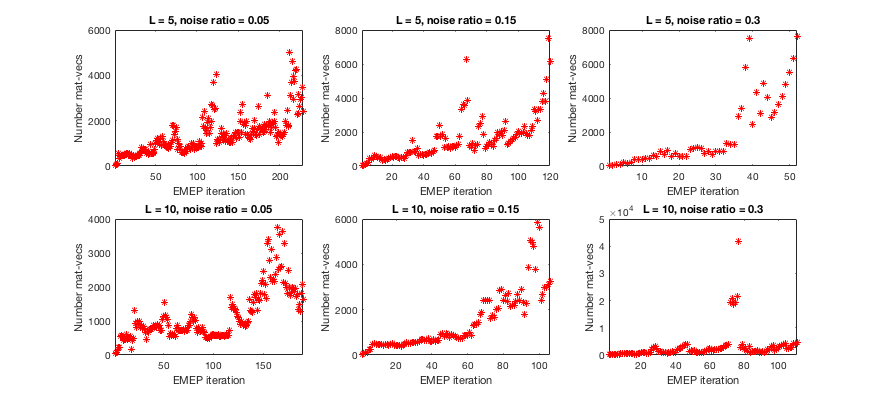
\includegraphics[scale=0.6]{EMEP_costs_num_mat_vecs} }\vspace{-0.4cm}
	\caption{Number of matrix-vector products for each iteration in the \emep \ for the six smaller models from Table \ref{Tab:EMEP_costs}	.}
\label{Fig:EMEP_costs_num_mat_vecs}
\end{figure}
% experiments.figure.noisyimage_costs

Figure \ref{Fig:EMEP_costs_num_mat_vecs} demonstrates that the number of matrix-vector products required for each \emep \ iterate varies greatly from earlier to later iterates.  
In each model, the later iterates account for the majority of the computational cost of the \emep.  
Additionally, some iterates require far more matrix-vector products than others (e.g., the iterates around $k=75$ in the bottom-right plot).
To help explain this change in computational costs, we now proceed to examine how the spectrum of the EMEP evolves.



\subsection{Evolving Spectrum Distribution} 	\label{Subsubsec:evol_mats-EMEP_spectrum_and_clustering}


We close this section by examining the evolving spectrum distribution of the \emep.
We find that the algebraically largest eigenvalues begin to cluster for  later EMEP iterates, likely causing those eigenvalue problems to be more difficult.
First, we examine the full spectrum of a few EMEP matrix iterates in Figure \ref{Fig:EMEP_full_spectrum}.




\begin{figure}[H]
\centering
\hbox{\hspace{-1.9cm} 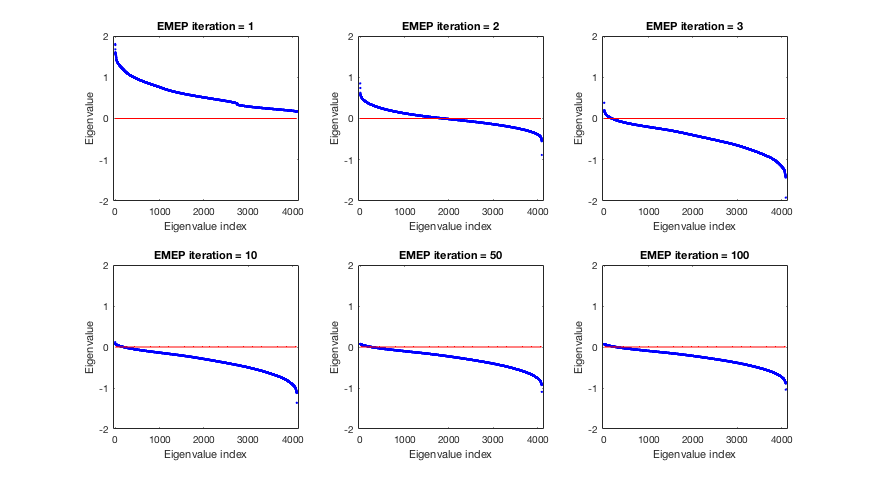
\includegraphics[scale=0.6]{EMEP_full_spectrum} }\vspace{-0.4cm}
	\caption{Spectrum of specific \emep \ matrix iterates $A_k$ for the model from Table \ref{Tab:EMEP_costs} with signal size $n = 4,096$, oversampling $L = 5$, and noise ratio $\epsilon_\text{rel} = 0.15$.}
\label{Fig:EMEP_full_spectrum}
\end{figure}
% experiments.figure.noisyimage_spectrumdist

As we see in Figure \ref{Fig:EMEP_full_spectrum}, the spectrum of the matrix iterates $A_k$ in the \emep \ shifts from completely positive for $A_1$ to mostly negative for later iterates.  This shift in spectrum is a consequence of optimizing the PLGD model (\ref{Eqn:PhaseLift-P-GD}).  The first matrix iterate $A_1 = \caA^*b$ will always be positive-semidefinite because the components of the observation $b=[b_1; b_2; \ldots; b_L]$ are all nonnegative and thus for all $x$ we have 
\[
x^*[\caA^*b]x 
	= \sum\limits_{\substack{j=1}}^{\substack{L}}
		[FC_jx]^* \textnormal{Diag}(b_j) F C_jx
	\geq 0.
\]
Since Algorithm \ref{Alg:PGD} minimizes the objective function $\lambda_1(\caA^*y_k)$, the algebraically largest eigenvalue $\lambda_1^{(k)}$ of $\caA^*y_k$ can be expected to decrease for later iterates $k$.  


As we will see in Section \ref{Subsec:evol_mats-IRAM}, the convergence rate of eigenvalue methods often depends on the distance between the desired eigenvalue $\lambda_j$ and the next algebraically largest eigenvalue $\lambda_{j+1}$.  Figure \ref{Fig:EMEP_largest_eigvals} depicts the 20 algebraically largest eigenvalues of the \emep \ iterates from Figure \ref{Fig:EMEP_full_spectrum}.


\begin{figure}[H]
\centering
\hbox{\hspace{-1.9cm} 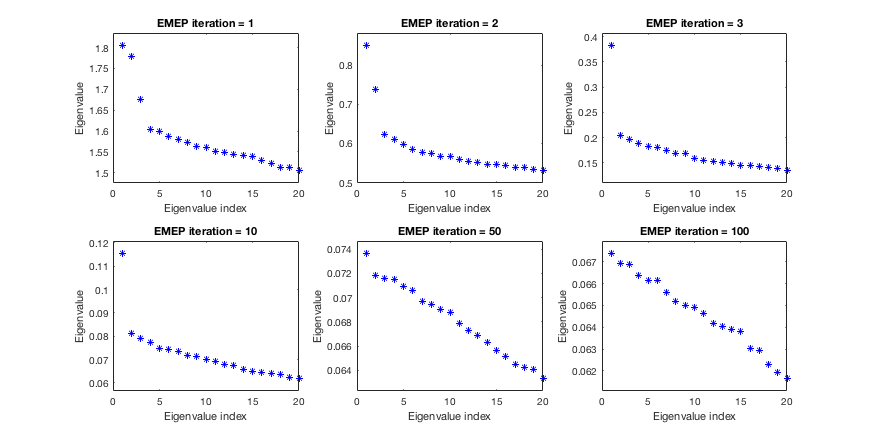
\includegraphics[scale=0.6]{EMEP_largest_eigvals} }\vspace{-0.4cm}
	\caption{Twenty algebraically largest eigenvalues of specific \emep \ matrix iterates $A_k$ for the model from Table \ref{Tab:EMEP_costs} with signal size $n = 4,096$, oversampling $L = 5$, and noise ratio $\epsilon_\text{rel} = 0.15$.}
\label{Fig:EMEP_largest_eigvals}
\end{figure}
% experiments.figure.noisyimage_spectrumdist

Figure \ref{Fig:EMEP_largest_eigvals} demonstrates that the algebraically largest eigenvalues of the matrix iterates $A_k$ cluster together as the \emep \ progresses.  
In general, this clustering in the \emep \ spectrum is expected.  
Section \ref{Subsec:PLGD_term_crit-stagnation} demonstrated that PLGD models with Gaussian noise (\ref{Eqn:PhaseLift-GD_Gaussian_noise}) typically have optimal primal matrices $X_\star$ with rank greater than one (see Table \ref{Tab:average_rank_soln_matrix_with_gaussian_dual_variable}).
And Corollary \ref{Cor:PLGD-optimality} (e) indicates that $\text{rank}(X_\star)$ is a lower bound on the multiplicity $r$ of the algebraically largest eigenvalue of the optimal dual matrix $\caA^*y_\star$.
Thus for later \emep \ iterates $k$, we can expect some $r$ algebraically largest eigenvalues $\lambda_1^{(k)}, \lambda_2^{(k)}, \ldots, \lambda_r^{(k)}$ to have a decreasing relative difference
\[
\frac{\lambda_i^{(k)} - \lambda_{i+1}^{(k)}}
	{\lambda_i^{(k)}}
\]
for $i = 1, 2, \ldots, r-1$.



The clustering of the algebraically largest eigenvalues as depicted in Figure \ref{Fig:EMEP_largest_eigvals} is known to slow the convergence rate of modern Krylov subspace methods.
Yet the choice of the parameters in these Krylov subspace methods can also affect their convergence rate significantly.
A thorough understanding of one such method (the implicitly restarted Arnoldi method) and its subroutines will help us to develop a new, adaptive strategy for choosing parameters for the \emep \ in Section \ref{Subsec:evol_mats-adaptive_IRAM}.






\section{The Implicitly Restarted Arnoldi Method}		\label{Subsec:evol_mats-IRAM}



% See following as references:
% http://www.cs.cornell.edu/~bindel/class/cs6210-f09/lec34.pdf
% http://people.inf.ethz.ch/arbenz/ewp/Lnotes/chapter11.pdf
%		Summarizes algorithms, math, convergence criteria, etc.
% ARPACK USERS GUIDE, p 53
%		Algo for IRAM on p 63

% Note: 
%	Prev	Golub
%	p		k, m
%	k		j
%	m		p (= m - j)
%	v		q


In this section we review the \textit{implicitly restarted Arnoldi method} (IRAM), a common large-scale eigenvalue method.  
First proposed by Sorensen \cite{sorensen1992implicit}, \cite{sorensen1997implicitly}, the IRAM is a combination of two essential algorithms.  
The \textit{$m$-step Arnoldi iteration} is used to build a matrix $Q_m$ of $m$ basis vectors which approximates the desired eigenspace.  
The \textit{$p$-step shifted QR iteration} restarts the matrix $Q_m$ with a specific strategy to damp unwanted eigenvalues, resulting in a smaller matrix $Q_j$ of $j<m$ basis vectors.  
Since the $m$-step Arnoldi iteration is an extension of the \textit{power method}, we first discuss the Power method before developing the IRAM.  
Altogether, the algorithms in this section are presented in the order depicted in Figure \ref{Fig:IRAM_flowchart}.

\begin{figure}[H] 
\centering
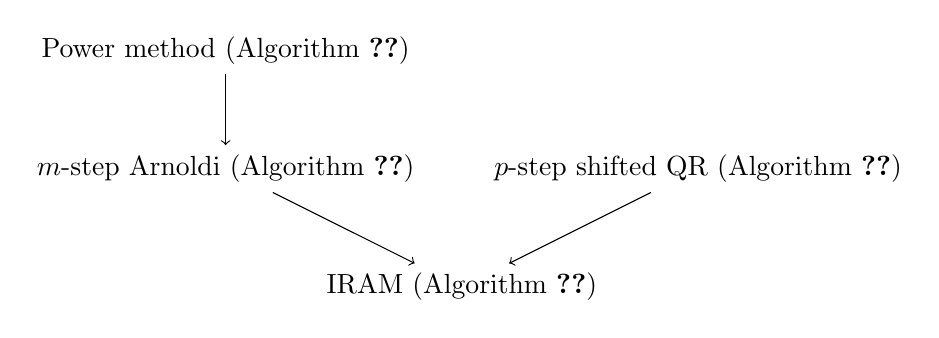
\begin{tikzpicture}
	\node (1) at (0,3) {Power method (Algorithm \ref{Alg:power_method})};
	\node (2) at (0,1.5) {$m$-step Arnoldi (Algorithm \ref{Alg:Arnoldi_iteration})};
	\node (3) at (6,1.5) {$p$-step shifted QR (Algorithm \ref{Alg:shifted_QR_iteration})};
	\node (4) at (3,0) {IRAM (Algorithm \ref{Alg:IRAM})};
	\draw[->] (1) -- (2);
	\draw[->] (2) -- (4);
	\draw[->] (3) -- (4);
\end{tikzpicture}
\caption{Dependency chart for the IRAM.}
\label{Fig:IRAM_flowchart}
\end{figure}

This section follows the treatment found in \cite[Chapters 8, 10]{golub2012matrix}, with occasional minor changes in notation.





\subsection{The Power Method} 			\label{Subsubsec:evol_mats-power_method}


The first method we consider is the \textit{power method}, a method for determining the largest magnitude eigenvalue $\lambda_1$ and corresponding eigenvector $v_1$ of a Hermitian matrix $A$.  The power method is based on the property that if $\lambda_1$ is strictly larger in magnitude than the next largest magnitude eigenvalue and the initial vector $q^{(0)}$ has a nonzero component in the direction of $v_1$ (i.e., $v_1^*q^{(0)} \neq 0$), then the sequence
\[
q^{(0)}, \frac{Aq^{(0)}}{||Aq^{(0)}||},  \frac{A^2q^{(0)}}{||A^2q^{(0)}||},  \frac{A^3q^{(0)}}{||A^3q^{(0)}||}, \ldots
\]
will have $v_1$ as its limit.  

Formally, Algorithm \ref{Alg:power_method} presents the power method as seen in \cite[Section 8.2.1]{golub2012matrix}.

\begin{algorithm}[H]
\caption{Power method}	\label{Alg:power_method}

\begin{algorithmic}[1]
	\Statex 	\textbf{Input:} Hermitian matrix $A$, initial approximate eigenvector $q^{(0)}$, relative tolerance $\textnormal{tol}_\textnormal{rel} > 0$.
	\Statex 	\textbf{Output:} Approximate largest magnitude eigenvalue $\lambda$ and the corresponding eigenvector $v$.
	\State		\textit{Initialize:} $q^{(0)} = q^{(0)}/||q^{(0)}||$, $\rho^{(0)} = [q^{(0)}]^*Aq^{(0)}$, $r^{(0)} = Au^{(0)} - \rho^{(0)}q^{(0)}$, $i= 1$.
	\While {\textit{not converged:} $ ||r^{(i)} || / (||Aq^{(i)}|| + |\rho^{(i)}|) > \textnormal{tol}_\textnormal{rel} $}
		\State		$z^{(i)} = Aq^{(i-1)}$
		\State		$q^{(i)} = z^{(i)} / ||z^{(i)}||$
		\State		$\rho^{(i)} = [q^{(i)}]^* z^{(i)}$
		\State		$r^{(i)} = Aq^{(i)} - \rho^{(i)}q^{(i)}$, $i = i + 1$
	\EndWhile
	\State		\textit{Return:} $(\lambda, v) = (\rho^{(i-1)} , q^{(i-1)})$.
\end{algorithmic}

\end{algorithm}


The simplicity of power method allows for insightful convergence results like the Theorem \ref{Thm:power_method_conv_rate}, in which we assume the matrix $A$ is real for clarity.

\begin{theorem}			\label{Thm:power_method_conv_rate}
Suppose $A \in \bbR^{n \times n}$ is symmetric with an eigenvalue decomposition
\[
V^*AV = \text{Diag}(\lambda_1, \lambda_2, \ldots, \lambda_n),
\]
where $V = [\ v_1 \ | \ v_2 \ | \cdots | \ v_n \ ]$ is orthogonal and $|\lambda_1| > |\lambda_2| \geq \cdots \geq |\lambda_n|$.  Let the vectors $q^{(i)}$ be generated by Algorithm \ref{Alg:power_method} and define $\theta_i \in [0, \pi/2]$ as 
\[
	\cos(\theta_i) = \left| v_1^Tq^{(i)} \right|.
\]
If $\cos(\theta_0) \neq 0$, then for $i = 0, 1, \ldots$ we have 
\begin{equation} 		\label{Eqn:power_method_conv_rate_1}
\left| \sin(\theta_i) \right| \leq \tan(\theta_0) \left| \frac{\lambda_2}{\lambda_1} \right|^i,
\end{equation}
\begin{equation} 		\label{Eqn:power_method_conv_rate_2}
\left| \lambda^{(i)} - \lambda_1 \right| \leq \max_{2 \leq j \leq n} \left| \lambda_1 - \lambda_i \right| \tan(\theta_0)^2 \left| \frac{\lambda_2}{\lambda_1} \right|^{2i}.
\end{equation}
\end{theorem}

\begin{proof}
See \cite[Theorem 8.2.1]{golub2012matrix}.
\end{proof}

Theorem \ref{Thm:power_method_conv_rate} establishes that the convergence rate of the power method (Algorithm \ref{Alg:power_method}) is dependent on the distance between $|\lambda_1|$ and $|\lambda_2|$.  If this distance $\epsilon = |\lambda_1| - |\lambda_2|$ is very small relative to $|\lambda_1|$, then we have
\[
\left| \frac{\lambda_2}{\lambda_1} \right| = \frac{|\lambda_1| - \epsilon}{|\lambda_1|} = 1 - \frac{\epsilon}{|\lambda_1|} \approx 1,
\]
and $|\sin(\theta_i)|$ in (\ref{Eqn:power_method_conv_rate_1}) may decreases very slowly.  







\subsection{The $m$-Step Arnoldi Iteration} 			\label{Subsubsec:evol_mats-Arnoldi}


The next method we consider is the \textit{$m$-step Arnoldi iteration} which extends the power method (Algorithm \ref{Alg:power_method}) to achieve a superior convergence rate.  An iteration of the power method generates a new approximate eigenvector ($q^{(i)}$ from steps 3 and 4) by normalizing the matrix-vector product of the previous vector.  In essence, the power method searches for the largest magnitude eigenvalue $\lambda_1$ and corresponding eigenvector $v_1$ of a matrix $A$ in the one-dimensional subspace $V = \textnormal{span} \{ Aq_1 \}$.  The $m$-step Arnoldi iteration extends the power method by searching for the Ritz pair (\ref{Def:Ritz_pair_val_vec}) ($\theta_1, u_1$) for $A$ with respect to the $m$-dimensional \textit{Krylov subspace}
\begin{equation}
\caK_m(A, q_1) = \textnormal{span}\{ q_1, Aq_1, A^2q_1, \ldots, A^{m-1}q_1 \}.
\label{Def:krylov_subspace}
\end{equation}
Algorithm \ref{Alg:Arnoldi_iteration} (as described in \cite[Algorithm 10.5.1]{golub2012matrix}) builds a unitary basis $Q_m$ of $\caK_m(A, q_1)$ which may be used to find the Ritz pair ($\theta_1, u_1$).
\begin{algorithm}[H]
\caption{$m$-step Arnoldi iteration}	\label{Alg:Arnoldi_iteration}

\begin{algorithmic}[1]
	\Statex		\textbf{Input:} Matrix $A \in \bbC^{n \times n}$, number of Arnoldi steps $m$, initial approximate eigenvector $q_1$.
	\Statex 	\textbf{Output:} Hessenberg matrix $H_m$, basis $Q_m$, residual $r_m$.
	\State		\textit{Initialize:} $q_1  = q_1 / ||q_1||$, \ \ $z = Aq_1$, \ \ $\alpha_1 = q_1^*z$, \ \ $r_1 = z - \alpha_1 q_1$, \ \ $Q_1 = [q_1]$, \ \ $H_1 = [\alpha_1]$.
	\For 			{$i = 1, \ldots, m-1$}
		\State	$\beta_i = ||r_i||$, \ \ $q_{i+1} = r_i / \beta_i$.
		\State	$Q_{i+1} = [Q_i \ | \ q_{i+1}]$, \ \ $\hat{H}_i = \begin{bmatrix}	H_i \\  \beta_i e_i^T	\end{bmatrix}$.
		\State	$z = Aq_{i+1}$.
		\State	$h = Q_{i+1}^*z$, \ \  $r_{i+1} = z - Q_{i+1}h$.
		\State	$H_{i+1} = [\hat{H}_i \ | \ h]$.
	\EndFor
	\State		\textit{Return:} $H_m, Q_m, r_m$.
\end{algorithmic}

\end{algorithm}

In order to obtain a Ritz pair ($\theta, u$) for $A$ with respect to $\caK_m(A, q_1)$, the $m$-step Arnoldi iteration generates an \textit{$m$-step Arnoldi decomposition}
\begin{equation} 		\label{Eqn:Arnoldi_decomp}
AQ_m = Q_m H_m + r_m e_m^*,
\end{equation}
where $H_m$ is an upper Hessenberg matrix.  If $(\theta, w)$ is an eigenpair for $H_m$ and $u = Q_mw$ then (\ref{Eqn:Arnoldi_decomp}) implies
\begin{equation} 			\label{Eqn:Arnoldi_decomp_Ritz_pairs}
(AQ_m - Q_mH_m)w = (A-\theta I) u = (e_m^*w)r_m.
\end{equation}
Additionally, steps 5 and 6 of Algorithm \ref{Alg:Arnoldi_iteration} indicate that $r_m$ is orthogonal to $\caK_m(A, q_1)$, and thus ($\theta, u$) is a Ritz pair for $A$ with respect to $\caK_m(A, q_1)$.  


The use of $\caK_m(A, q_1)$ in Algorithm \ref{Alg:Arnoldi_iteration} allows for superior convergence to Algorithm \ref{Alg:power_method}.  Note that the largest magnitude Ritz pair $(\theta_1, u_1)$ for $A$ with respect to $\caK_m(A, q_1)$ generated by Algorithm \ref{Alg:Arnoldi_iteration}  is guaranteed to be at least comparable to the $m$-th iterate of Algorithm \ref{Alg:power_method} since $A^{m-1}q_1 \in  \caK_m(A, q_1)$.  To compare the convergence rates of Algorithms \ref{Alg:power_method} and \ref{Alg:Arnoldi_iteration} more precisely, assume the matrix $A$ in real and symmetric.  Then the matrix $H_m$ returned by Algorithm \ref{Alg:Arnoldi_iteration} is tridiagonal and this algorithm is equivalent to the \textit{$m$-step Lanczos iteration} \cite[Algorithm 10.1.1]{golub2012matrix}.  In this case, we have the Theorem \ref{Thm:Lanczos_conv_rate}.  Note that this theorem involves \textit{Chebyshev polynomials} \cite[Section 4.4]{saad2011numerical}, a sequence of polynomials defined recursively as
\begin{equation} 			\label{Def:Chebyshev_polys}
c_k(x) = 2x c_{k-1}(x) - c_{k-2}(x)
\end{equation}
for $k \geq 2$, with $c_0 = 1$ and $c_2 = x$ .

\begin{theorem}   		\label{Thm:Lanczos_conv_rate}
Let $A \in \bbR^{n \times n}$ be symmetric with an eigenvalue decomposition
\[
V^*AV = \text{Diag}(\lambda_1, \lambda_2, \ldots, \lambda_n),
\]
where $V = [\ v_1 \ | \ v_2 \ | \cdots | \ v_n \ ]$ is orthogonal and $\lambda_1 \geq \lambda_2 \geq \cdots \geq \lambda_n$.  Suppose the $m$-step Arnoldi iteration (Algorithm \ref{Alg:Arnoldi_iteration}) is performed and $H_k$ is the tridiagonal matrix returned by this algorithm.  If $\theta_1$ is the algebraically largest eigenvalue of $H_m$, then
\begin{equation} 			\label{Eqn:Lanczos_thm_1}
\lambda_1 \geq \theta_1 \geq \lambda_1 - (\lambda_1 - \lambda_n) 
\left( \frac{\tan(\phi_1)}{c_{m-1}(1+2\rho_1)} \right)^2,
\end{equation}
where $\cos(\phi_1) = |q_1^Tv_1|$,
\begin{equation}		\label{Eqn:Lanczos_thm_2}
\rho_1 = \frac{\lambda_1 - \lambda_2}{\lambda_2 - \lambda_n},
\end{equation}
and $c_{m-1}(x)$ is the Chebyshev polynomial of degree $m-1$.
\end{theorem}

\begin{proof}
See \cite[Theorem 10.1.2]{golub2012matrix}.
\end{proof}

The convergence rate established in Theorem \ref{Thm:Lanczos_conv_rate} may also be applied to Algorithm \ref{Alg:power_method}, giving the Corollary \ref{Cor:Lanczos_cor_for_power_method}.

\begin{corollary} 			\label{Cor:Lanczos_cor_for_power_method}
Let $A \in \bbR^{n \times n}$ be symmetric and positive semidefinite with an eigenvalue decomposition
\[
V^*AV = \text{Diag}(\lambda_1, \lambda_2, \ldots, \lambda_n),
\]
where $V = [\ v_1 \ | \ v_2 \ | \cdots | \ v_n \ ]$ is orthogonal and $\lambda_1 \geq \lambda_2 \geq \cdots \geq \lambda_n \geq 0$.  Suppose $m$ steps of the power method (Algorithm \ref{Alg:power_method}) are performed and $\gamma_1 = \rho^{(m)}$ is the returned Ritz value.  Then
\begin{equation} 			\label{Eqn:Lanczos_cor_for_power_method}
\lambda_1 \geq \gamma_1 \geq \lambda_1 - (\lambda_1 - \lambda_n) 
\tan^2(\phi_1) \left( \frac{\lambda_2}{\lambda_1} \right)^{2(m-1)},
\end{equation}
where $\cos(\phi_1) = |q_1^Tv_1|$.
\end{corollary}

\begin{proof}
See \cite[Theorem 10.1.2]{golub2012matrix} and replace the Chebyshev polynomial in this proof with $p(x) = x^{k-1}$.
\end{proof}


The lower bounds in Theorem \ref{Thm:Lanczos_conv_rate} and Corollary \ref{Cor:Lanczos_cor_for_power_method} may be used to compare the expected convergence rates for Algorithms \ref{Alg:power_method} and \ref{Alg:Arnoldi_iteration}.  The following comparison is based on \cite[Section 10.1.6]{golub2012matrix}.  Assume $A \in \bbR^{n \times n}$ is symmetric and also positive semidefinite for clarity.  Assume Algorithms \ref{Alg:power_method} and \ref{Alg:Arnoldi_iteration} have been run for $m$ steps with the same initial vector $q_1$.  Let $\gamma_1 = \rho^{(m)}$ be the Ritz value for $A$ generated by step 5 of Algorithm \ref{Alg:power_method}.  And let $\theta_1$ be the Ritz value for $A$ with respect to $\caK_m(A, q_1)$ generated by the algebraically largest eigenvalue of $H_m$ from Algorithm \ref{Alg:Arnoldi_iteration}.  Then we may compare the lower bounds (\ref{Eqn:Lanczos_cor_for_power_method}) for $\gamma_1$ and (\ref{Eqn:Lanczos_thm_1}) for $\theta_1$ by comparing the values
\begin{equation} 		\label{Eqn:power_method_lower_bound}
P_{m-1} = \left( \frac{\lambda_2}{\lambda_1} \right)^{2(m-1)},
\end{equation}
\begin{equation}  	\label{Eqn:Lanczos_lower_bound}
L_{m-1} 
	= \frac{1}{\left[c_{m-1}\left(2\frac{\lambda_1}{\lambda_2} -1 \right)\right]^2} 
	\geq 	\frac{1}{\left[ c_{m-1}\left( 1 + 2 \rho_1 \right) \right]^2}.
\end{equation}
Table \ref{Tab:Lanczos_vs_power_method} compares $P_{m-1}$ and $L_{m-1}$ for a few values of $m$ and $\lambda_1/\lambda_2$.

\begin{table}[H]
\centering
\begin{tabular}{ |c|cc|cc| }
 \hline

 	&	\multicolumn{2}{c|}{$m = 10$}
 		&	\multicolumn{2}{c|}{$m = 20$}	\\
 $\lambda_1 / \lambda_2$	&	$P_{m-1}$	&	$L_{m-1}$
 		&	$P_{m-1}$	&	$L_{m-1}$		\\ 			
 \hline
$1.10$
	&	$1.8 \times 10^{-1}$ & $5.5 \times 10^{-5}$
		&	$2.7 \times 10^{-2}$ & $2.1 \times 10^{-10}$	\\
$1.01$
	&	$8.4 \times 10^{-1}$ & $1.0 \times 10^{-1}$
		&	$6.9 \times 10^{-1}$ & $2.0 \times 10^{-3}$	\\
 \hline
\end{tabular}
\caption{Lower bound terms (\ref{Eqn:power_method_lower_bound}) and (\ref{Eqn:Lanczos_lower_bound}) for Ritz values generated by Algorithms \ref{Alg:power_method} and \ref{Alg:Arnoldi_iteration} } \label{Tab:Lanczos_vs_power_method}
\end{table}

Table \ref{Tab:Lanczos_vs_power_method} demonstrates that the use of the Krylov subspace $\caK_m(A, 	q_1)$ in Algorithm \ref{Alg:Arnoldi_iteration} allows for superior convergence to Algorithm \ref{Alg:power_method}.  Yet this superior convergence rate is slowed somewhat when the desired eigenvalue $\lambda_1$ is close to $\lambda_2$.  For eigenvalue problems where the value $\lambda_1 / \lambda_2$ is very small (like later iterates of the \emep, as demonstrated in Figure \ref{Fig:EMEP_largest_eigvals}), we may seek to increase the number of steps $m$ in Algorithm \ref{Alg:Arnoldi_iteration}.  Yet increasing $m$ can be computationally prohibitive if the eigenvalue problem is very large, requiring significant memory to store $Q_m$ and significant computation to compute the eigenvalue decomposition of $H_m$.






\subsection{The $p$-Step Shifted QR Iteration} 			\label{Subsubsec:evol_mats-QR_iteration}


To take advantage of the convergence rate of Algorithm \ref{Alg:Arnoldi_iteration} for larger eigenvalue problems, the Arnoldi decomposition (\ref{Eqn:Arnoldi_decomp}) may be restarted with the \textit{$p$-step shifted QR iteration} developed by \cite{sorensen1992implicit} and discussed in \cite[Sections 10.5.2-3]{golub2012matrix}.  To develop this algorithm, assume we are seeking the $j$ algebraically largest eigenvalues of a Hermitian matrix $A \in \bbC^{n \times n}$ and we require that the $m$-step Arnoldi decomposition (\ref{Eqn:Arnoldi_decomp}) $AQ_m = Q_m H_m + r_m e_m^*$ has a fixed size $m > j$.  First we run Algorithm \ref{Alg:Arnoldi_iteration} with the initial vector $q_1$ to obtain $AQ_m = Q_m H_m + r_m e_m^*$.  Next, recall that the matrix $H_m$ may be used to identify the desired Ritz pairs $\{(\theta_i, u_i)\}_{i=1}^j$ for $A$ with respect to $\caK_m(A, q_1)$, as described in (\ref{Eqn:Arnoldi_decomp_Ritz_pairs}).  Yet $H_m$ also contains Ritz values $\theta_{j+1}, \ldots, \theta_m$ which correspond to unwanted eigenvalues of $A$.  To damp these unwanted Ritz values, we may select an appropriate degree $p = m-j$ filter polynomial $p(\lambda)$.  The $p$-step shifted QR iteration uses the filter polynomial
\begin{equation} 			\label{Eqn:filter_poly}
p(\lambda) = c \cdot (\lambda - \mu_1) (\lambda - \mu_2) \cdots (\lambda - \mu_p),
\end{equation}
where $c$ is a constant and the shift values $\mu_1 = \theta_{j+1}, \ldots, \mu_p = \theta_m$ are the $p$ unwanted Ritz values of $A$ with respect to $\caK_m(A, q_1)$.  Algorithm \ref{Alg:shifted_QR_iteration} (as described in \cite[Section 10.5.3]{golub2012matrix}) uses the filter polynomial (\ref{Eqn:filter_poly}) implicitly by applying $p$ shifted QR steps to $H_m$.
%(see \cite[Section 5.2]{golub2012matrix} for details regarding the QR factorization)
\begin{algorithm}[H]
\caption{$p$-step shifted QR iteration (implicit polynomial filtering)}	\label{Alg:shifted_QR_iteration}

\begin{algorithmic}[1]
	\Statex 	\textbf{Input:} Hessenberg matrix $H_m \in \bbC^{m \times m}$ and shift values $\mu_1, \ldots, \mu_p$.
	\Statex 	\textbf{Output:} Processed Hessenberg matrix $H_m^+ \in \bbC^{m \times m}$ and change of basis $V \in \bbC^{m \times m}$, with $H_m^+ = V^*H_mV$.
	\State		Set $H^{(0)} = H_m$.
	\For {$i = 1, \ldots, p$ }
		\State		\textit{QR factorization:} $H^{(i-1)} - \mu_i I = V_iR_i$.
		\State		\textit{Update:} $H^{(i)} = R_iV_i + \mu_iI$.
	\EndFor
	\State		Set $H_m^+ = H^{(p)}$, $V = V_1  V_2 \cdots V_p$.
	\State		\textit{Return:} $H_m^+, V$.
\end{algorithmic}

\end{algorithm}

Proposition \ref{Prop:Arnoldi_restart} establishes that Algorithm \ref{Alg:shifted_QR_iteration} implicitly applies the filter polynomial $p(\lambda)$ from (\ref{Eqn:filter_poly}) to the initial vector $q_1$ used to create the $m$-step Arnoldi decomposition (\ref{Eqn:Arnoldi_decomp}).

\begin{prop} 			\label{Prop:Arnoldi_restart}
Let $A \in \bbC^{n \times n}$ be Hermitian and $AQ_m = Q_mH_m + r_me_m^*$ be the $m$-step Arnoldi decomposition (\ref{Eqn:Arnoldi_decomp}) returned by Algorithm \ref{Alg:Arnoldi_iteration} with initial vector $q_1$.  And let $\mu_1, \ldots, \mu_p$ be the $p$ smallest algebraic eigenvalues of $H_m$.  Run Algorithm \ref{Alg:shifted_QR_iteration} with $H_m$ and $\mu_1, \ldots, \mu_p$ as inputs, and return $H_m^+$, $V = V_1 \cdots V_p$, and $R = R_p \cdots R_1$.

Then the restarted matrix $Q_+ = Q_mV$ will have the first column
\[
q_+ = Q_mV(:,1) = p(A)q_1,
\]
where $p(\lambda)$ is the filter polynomial (\ref{Eqn:filter_poly}) with constant $c = 1/R(1,1)$.
\end{prop}


\begin{proof}
See \cite[Section 10.5.3]{golub2012matrix}.
\end{proof}


\iffalse

\begin{proof}
First we must show that 
\begin{equation} 		\label{Eqn:filter_poly_proposition-VR}
VR = (H_m - \mu_1I) \cdots (H_m - \mu_pI).
\end{equation}

Using induction, we see that if $p=1$ then clearly (\ref{Eqn:filter_poly_proposition-VR}) holds.  If $p>1$, then let $\tilde{V}=V_1 \cdots V_{p-1}$ and $\tilde{R} = R_{p-1} \cdots R_1$, and note that $H^{(p-1)} = \tilde{V}^*H_m\tilde{V}$.  Then we have
\[
\begin{split}
VR & = \tilde{V}(V_pR_p)\tilde{R} 
	= \tilde{V} \left( H^{(p-1)} - \mu_pI \right) \tilde{R}
	= \tilde{V}\left( \tilde{V}^*H_m \tilde{V} - \mu_p I \right)\tilde{R}	\\
	& = \left(H_m - \mu_p I \right) \tilde{V}\tilde{R}
	= (H_m - \mu_p I) (H_m - \mu_1 I) \cdots (H_m - \mu_{p-1}I) 	\\
	&=  (H_m - \mu_1I) \cdots (H_m - \mu_pI),
\end{split}
\]
and (\ref{Eqn:filter_poly_proposition-VR}) holds.

Next, note that if the $m$-step Arnoldi decomposition (\ref{Eqn:Arnoldi_decomp}) is right-multiplied by $e_1$, then for all $\mu$ we have
\begin{equation} 			\label{Eqn:filter_poly_propostion-flip}
\left(A - \mu I \right)Q_me_1 = Q_m \left(H_m - \mu I \right) e_1.
\end{equation}

Then we have
\[
\begin{split}
q_+ 
	& = Q_mV(:,1) = Q_m \left[ \frac{1}{R(1,1)}VR e_1 \right] 	\\
	& 	= Q_m p(H_m) e_1 = p(A)Q_m e_1	\\
	& 	= p(A) q_1,
\end{split}
\]
where the third equality is given by (\ref{Eqn:filter_poly_proposition-VR}) and the fourth is given by (\ref{Eqn:filter_poly_propostion-flip}).
\end{proof}

\fi





After performing Algorithm \ref{Alg:shifted_QR_iteration}, we have the transformed $m$-step Arnoldi decomposition (\ref{Eqn:Arnoldi_decomp})
\begin{equation}			\label{Eqn:Arnoldi_decomp_transf_shifted_QR}
AQ_+ = Q_+H_+ + r_me_m^*V,
\end{equation}
where $V = V_1 \cdots V_p$ from Algorithm \ref{Alg:shifted_QR_iteration} and $Q_+ = Q_mV$.  As a consequence of the QR steps used in Algorithm \ref{Alg:shifted_QR_iteration}, we can also show that the first $j = m-p$ columns of (\ref{Eqn:Arnoldi_decomp_transf_shifted_QR}) form a new $j$-step Arnoldi decomposition.  Note that $V_1, \ldots, V_p$ are all upper Hessenberg due to the QR factorization in step 3 of Algorithm \ref{Alg:shifted_QR_iteration}.  Then $V$ has a lower band $p$ and $V(m, 1:m-p-1) = V(m, 1:j-1) = 0$, giving
\begin{equation} 			\label{Eqn:Arnoldi_decomp_transf_shifted_QR-part1}
r_me_m^*V(:, 1:j) = V(m,j)r_me_j^*.
\end{equation}
Also, $H_+$ is upper Hessenberg and thus $H_+(j+1:m, 1:j) = H_+(j+1,j)e_1e_j^*$, giving
\begin{equation} 		\label{Eqn:Arnoldi_decomp_transf_shifted_QR-part2}
\begin{split}
Q_+H_+(:, 1:j) 
	&	=  Q_+(:, 1:j) H_+(1:j, 1:j) + Q_+(:, j+1:m)H_+(j+1:m, 1:j) \\
	&	=	Q_+(:, 1:j) H_+(1:j, 1:j) +  H_+(j+1,j)Q_+(:,j+1)e_j^*.
\end{split}
\end{equation}

Therefore, if we set $Q_j = Q_+(:, 1:j) = Q_mV(:, 1:j)$, $H_j = H_+(1:j, 1:j)$, and $r_j = V(m,j)r_m + H_+(j+1,j)Q_+(:,j+1)$, then equations (\ref{Eqn:Arnoldi_decomp_transf_shifted_QR}-\ref{Eqn:Arnoldi_decomp_transf_shifted_QR-part2}) give the new $j$-step Arnoldi decomposition
\begin{equation}		\label{Eqn:Arnoldi_decomp_j-step_update}
\begin{split}
AQ_j  
	&	= AQ_+(:, 1:j) 	\\
	& = Q_+(:, 1:j)H_+(1:j, 1:j) + \left[V(m,j)r_m + H_+(j+1,j)Q_+(:,j+1) \right] e_j^*		\\
	& = Q_jH_j + r_je_j^*,
\end{split}
\end{equation}
and we may resume Algorithm \ref{Alg:Arnoldi_iteration} at step $j+1$.




\subsection{The Implicitly Restarted Arnoldi Method} 			\label{Subsubsec:evol_mats-IRAM}


Combining Algorithms \ref{Alg:Arnoldi_iteration} and \ref{Alg:shifted_QR_iteration} as described above, we have Algorithm \ref{Alg:IRAM} as presented in \cite[Section 10.5.3]{golub2012matrix}.

\begin{algorithm}[H]
\caption{Implicitly restarted Arnoldi method (IRAM)}	\label{Alg:IRAM}

\begin{algorithmic}[1]
	\Statex 	\textbf{Input:} Matrix $A \in \bbC^{n \times n}$, initial approximate eigenvector $q_1$, number of requested algebraically largest eigenvalues $j$, maximum Arnoldi decomposition (\ref{Eqn:Arnoldi_decomp}) size $m$.
	\Statex 	\textbf{Output:} Approximate algebraically largest eigenpairs $(\Lambda_j, V_j)$.
	\State		\textit{Initialize with Algorithm \ref{Alg:Arnoldi_iteration}:} Perform the $m$-step Arnoldi iteration with initial vector $q_1$ to obtain $AQ_m = Q_m H_m + r_m e_m^*$.
	\While {not converged}
		\State		Compute the eigenvalues $\theta_1, \ldots , \theta_m$ of $H_m$ and identify the $p = m-j$ (unwanted) shift values $\mu_1 = \theta_{j+1},  \ldots, \mu_p = \theta_m$.
		\State		\textit{Algorithm \ref{Alg:shifted_QR_iteration}:}  Perform the $p$-step shifted QR iteration to obtain the Hessenberg matrix $H_+$ and change of basis $V$.
		\State		\textit{Restart the Arnoldi factorization:} Set 
		$Q_j = Q_mV(:, 1:j)$,
		$H_j = H_+(1:j, 1:j)$,
		and $r_j = V(m,j)r_m + H_+(j+1,j)Q_+(:,j+1)$ per (\ref{Eqn:Arnoldi_decomp_j-step_update}).
		\State		\textit{Algorithm \ref{Alg:Arnoldi_iteration}:}  Beginning with $AQ_j = Q_jH_j + r_je_j^*$, perform steps $j+1, \ldots, m$ of the Arnoldi iteration to obtain $AQ_m = Q_m H_m + r_m e_m^*$.
	\EndWhile
	\State 		Compute the $j$ algebraically largest eigenvalues $\Lambda_j = \{ \lambda_1, \ldots, \lambda_j\}$ and corresponding eigenvectors $u_1, \ldots, u_j$ of $H_m$.  Set $V_j = [ \ Q_m u_1 \ | \cdots | \ Q_m v_j \ ]$.
	\State		\textit{Return:} $(\Lambda_j, V_j)$.
\end{algorithmic}

\end{algorithm}


The IRAM is the eigenvalue method we use in Section \ref{Subsec:evol_mats-adaptive_IRAM} to handle the \emep.  The choice of parameters $m$ (the Arnoldi decomposition size) and $j$ (number of requested eigenvalues) can greatly impact the efficiency of IRAM (see Section \ref{Subsec:evol_mats-adaptive_IRAM}).  For many large-scale eigenvalue problems, the IRAM is a very effective and convenient method.  Due to the implicit polynomial filtering in step 4 of IRAM, this method is particularly effective when the $j$ algebraically largest eigenvalues have modest separation from $\lambda_{j+1}$.  And since the IRAM only has two parameter choices, there is little optimization required by the user.

However, when $\lambda_j \approx \lambda_{j+1}$ and the Arnoldi decomposition size $m$ is not sufficiently large, the IRAM may require many iterations to achieve the desired tolerance. 
 As we will see in Section \ref{Subsec:evol_mats-adaptive_IRAM}, the appropriate choice of $m$ and $j$ in this circumstance may make the IRAM far more competitive.  
Yet choosing $m$ and $j$ without prior knowledge of the eigenvalue distribution is inherently heuristic.  
Additionally, if the inputted matrix $A$ is very large, then it may be prohibitive to store the $Q_m \in \bbC^{n \times m}$ in active memory.  In particular, if the image or signal $x$ being recovered in the PLGD problem has $n$ pixels, then $Q_m$ will require $m-$times as much storage space.  
Thus we proceed in the next section by considering an alternative Krylov subspace method which does not require parameter tuning, nor a large subspace to be held in memory.


Note that the IRAM is implemented in the numerical software package \texttt{ARPACK} (the ARnoldi PACKage) in FORTRAN 77 \cite{lehoucq1998arpack}.  Many numerical computing environments include large-scale eigenvalue methods which having bindings to ARPACK, including \texttt{eigs} in MATLAB, \texttt{eigs} and \texttt{eigsh} in the Python package SciPy, \texttt{eigs} in R, and \texttt{eigs} in the Julia package Arpack.jl. 







\section{A New Strategy for the EMEP}
\label{Subsec:evol_mats-adaptive_IRAM}


In this section we develop a new strategy which uses the IRAM (Algorithm \ref{Alg:IRAM}) to handle the \emep \ while adaptively changing one of the IRAM parameters based on the results from the previous EMEP iterates.
As discussed in Section \ref{Subsec:evol_mats-IRAM}, the IRAM has only two key parameters: the number of requested eigenvalues $r$ and the Arnoldi decomposition (\ref{Eqn:Arnoldi_decomp}) size $m$.
As we will see, the proper choice of these parameters can greatly reduce the number of matrix-vector products required for the EMEP.


We begin by examining the change in computational costs  (as measured by matrix-vector products) with respect to various \emep \ iterates $k$ and IRAM parameters $r$ in Figure \ref{Fig:Numerics-num_matvecs_orig_vs_optimal_params}.
In the original implementation of Algorithm \ref{Alg:PGD}, all EMEP iterates were handled using the IRAM with $r=2$ requested eigenvalues and Arnoldi decomposition size $m = \min \{  \max \{ 2r, 20 \}, n \}$, where $n$ is the size of the desired signal $x$.  
This choice of $m$ is equivalent to the default parameter setting in the IRAM solver \texttt{eigs} for MATLAB and evaluates to $m=20$ for $n \geq 20$.
Yet the plots in Figure \ref{Fig:Numerics-num_matvecs_orig_vs_optimal_params} demonstrate that choosing a fixed parameter $r=2$ can result in far more matrix-vector products than is optimal.


\begin{figure}[H]
\centering
\hbox{\hspace{-0.8cm} 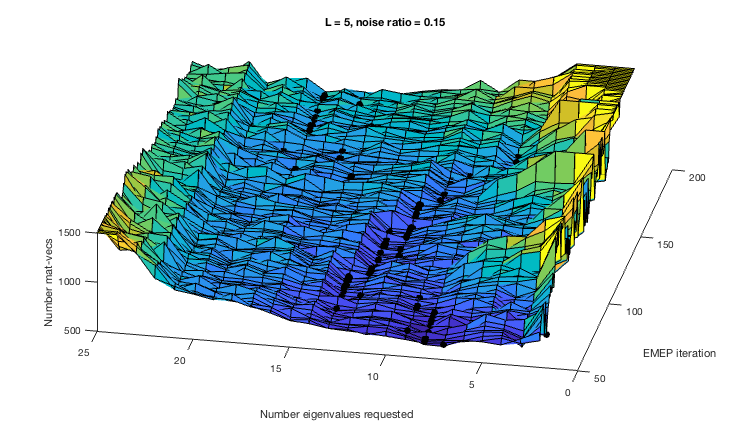
\includegraphics[scale=0.6]{Numerics-num_matvecs_orig_vs_optimal_params_1} }\vspace{1.0cm}
\hbox{\hspace{-1.6cm} 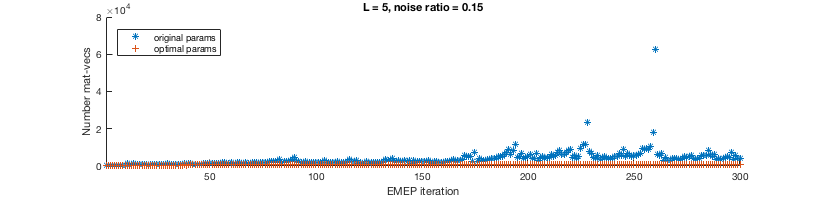
\includegraphics[scale=0.6]{Numerics-num_matvecs_orig_vs_optimal_params_2} }\vspace{0.0cm}
	\caption{
Performance results for an EMEP from a PLGD model with Gaussian noise	(\ref{Eqn:PhaseLift-GD_Gaussian_noise}) with noise ratio $\epsilon_\text{rel} = 0.15$, oversampling rate $L = 5$, and original signal from Figure \ref{Fig:parrot_signal_iterates} resized to $64 \times 64$ pixels.
Top: Number of matrix-vector products (capped at 1,500 for better viewing) for various EMEP iterates and number of requested eigenvalues $r$.  
Arnoldi decomposition size is set to $m = 40$ and black dots indicate the optimal parameter $r$ with the minimum number of products for each EMEP iterate.
Bottom: Plot of IRAM results for the EMEP with optimal parameters from top plot and fixed parameters $r=2$ and $m=20$.
	}
\label{Fig:Numerics-num_matvecs_orig_vs_optimal_params}
\end{figure}
% experiments.figure.noisyimage_adaptive_eig_full_exp




We now examine Figure \ref{Fig:Numerics-num_matvecs_orig_vs_optimal_params} to develop an adaptive strategy for choosing the number of requested eigenvalues $r$ for the sequence of EMEP iterates.
The top plot in Figure \ref{Fig:Numerics-num_matvecs_orig_vs_optimal_params} shows that the optimal choice of parameter $r$ typically changes only slightly between EMEP iterates.
However, the optimal parameter $r$ can increase quickly for later EMEP iterates (as we see around iterate 150 in the top plot in Figure \ref{Fig:Numerics-num_matvecs_orig_vs_optimal_params}).
Based on these observations, we may develop a strategy for choosing a sequence of parameters $r_1, r_2, \ldots, r_{maxit}$ as follows.
In order to measure change in the number of matrix-vector products for each iterate, we require that each pair of parameters $r_{k-1}$ and $r_k$ differ by at least one.
To select a new parameter $r_+$, we compare the two most recent choices for $r$ and the resulting number of matrix-vector products.
If these two choices for $r$ decreased the number of matrix-vector products, we continue to shift the value of $r$ in this direction by one unit; and otherwise we shift $r$ in the opposite direction.
We also allow $r$ to increase or decrease $r$ more rapidly by comparing the four most recent choices for $r$ and the resulting number of matrix-vector products using linear interpolation.
If these recent choices suggest the same shift as the first comparison, then we shift $r$ in this direction by two units rather than one.



This adaptive strategy for choosing the number of requested eigenvalues $r_k$ for each \emep \ iterate $k$ has the following steps.
First, we select a fixed Arnoldi decomposition size $m$ and initialize $r_1=r_{min}$ and $r_2 = r_1+1$ (where $r_{min}=2$, and $r_{max} = \min\{ 30, m-5 \}$, and we set the default value $m=40$).  
At each step $k \geq 2$ we update $r_{k+1} =  r_k + \delta$, where $\delta \in \{-2, -1, 1, 2\}$ is a shift based on the number of requested eigenvalues $r_k, r_{k-1}, \ldots$ and number of matrix-vector products $t_k, t_{k-1}, \ldots$ for the previous eigenvalues problems.
The shift $\delta$ is computed as follows.
First, we determine a \textit{$2$-step shift value} $\delta_2 \in \{-1, 1\}$ based on $r_{k-1}, r_k$ and $t_{k-1}, t_k$.
If $r_k > r_{k-1}$ and $t_k < t_{k-1}$ then the number of matrix-vector products in the \emep \ decreased as the number of requested eigenvalues was increased, suggesting we should shift $r_k$ by $\delta_2 = 1$.
By the same reasoning for the other three inequality cases, we define the
\textit{$2$-step shift value} as
\begin{equation}				\label{Eqn:adaptive_delta_2}
\delta_2 = \sign(r_k - r_{k-1}) \cdot \sign(t_{k-1} - t_k),
\end{equation}
where $\sign(0)$ is defined as $1$.
Next, if $k \geq 4$ then we compute a linear interpolation of the past four requested eigenvalue numbers and matrix-vector products by solving
\begin{equation} 			\label{Eqn:adaptive_delta_4_lin_interp_prob}
\min_{\alpha, \beta} || y - \alpha e - \beta x ||,
\end{equation}
where $y = [t_{k-3}; t_{k-2}; t_{k-1}; t_k]$ is the vector of matrix-vector product values, $x = [r_{k-3}; r_{k-2}; r_{k-1}; r_k]$ is the vector of the number of requested eigenvalues, and $e = [1;1;1;1]$.
If the solution to (\ref{Eqn:adaptive_delta_4_lin_interp_prob}) has $\beta > 0$ then the past four eigenvalue problems suggest that $t_i$ increases with $r_i$, and thus we should decrease $r_k$.
Thus we have the \textit{$4$-step shift value}
\begin{equation}			\label{Eqn:adaptive_delta_4}
\delta_4 = -\sign(\beta),
\end{equation}
where $\beta$ is determined by (\ref{Eqn:adaptive_delta_4_lin_interp_prob}).
If $\delta_2 = \delta_4$, then the $2$-step (\ref{Eqn:adaptive_delta_2}) and $4$-step equations (\ref{Eqn:adaptive_delta_4}) both suggest we should shift in the direction of $\delta_2$, and we select the shift $\delta = 2\delta_2$.
If $\delta_2 \neq \delta_4$ then we rely on the $2$-step equation (\ref{Eqn:adaptive_delta_2}) and select the shift value $\delta = \delta_2$.
Finally, if $r_k = r_{min}$ then we set $\delta = 1$ and if $r_k = r_{max}$ the we set $\delta = -1$.
Altogether, these steps lead to \textit{the IRAM with adaptive parameter selection} for the \emep.



\begin{algorithm}[H]
\caption{The IRAM with adaptive parameter selection for the \emep}	\label{Alg:adaptive_IRAM}

\begin{algorithmic}[1]
	\Statex 	\textbf{Input:} Sequence of matrices $\{ A_k \}_{k=1}^{maxit}$ from the \emep, Arnoldi decomposition (\ref{Eqn:Arnoldi_decomp})  size $m$ (default parameter $m = 40$).
	\Statex 	\textbf{Output:} \emep \ solution eigenpairs $\{ (\lambda_1^{(k)}, v_1^{(k)}) \}_{k=1}^{maxit}$ and  $\{ (\lambda_2^{(k)}, v_2^{(k)}) \}_{k=1}^{maxit}$.
	\State		\textit{Initialize:} $r_{min}=2$, $r_{max} = \min\{ 30, m-5 \}$, $r_1=r_{min}$, $t_0=-1$, $k=1$.
	\While {$k \leq maxit$}
		\State		\textit{Algorithm \ref{Alg:IRAM}:} Perform IRAM with matrix $A_k$, number of requested algebraically largest eigenvalues $r_k$, and maximum Arnoldi decomposition size $m$.  Return eigenpairs $(\lambda_1^{(k)}, v_1^{(k)} )$, $(\lambda_2^{(k)}, v_2^{(k)} )$ and number of matrix-vector products $t_k$.
		\If		{$r_k = r_{min}$}
			\State 		$r_{k+1} = r_k + 1$
		\ElsIf 	{$r_k = r_{max}$}
			\State		$r_{k+1} = r_k - 1$
		\ElsIf	{$k < 4$}
			\State		Compute $2$-step shift value $\delta_2$ from (\ref{Eqn:adaptive_delta_2}) and set $\delta = \delta_2$
			\State		$r_{k+1} = r_k + \delta$
		\Else
			\State 		Compute $2$-step shift value $\delta_2$ from (\ref{Eqn:adaptive_delta_2}) and $4$-step shift value $\delta_4$ from (\ref{Eqn:adaptive_delta_4})
			\If						{$\delta_2 = \delta_4$}
				\State		Set $\delta = 2\delta_2$
			\Else
				\State 			Set $\delta = \delta_2$
			\EndIf
			\State		$r_{k+1} =\min \{ \max \{ r_k + \delta, r_{min} \}, r_{max} \}$
		\EndIf
		\State		$k = k+1$
	\EndWhile
	\State		\textit{Return:} $\{ (\lambda_1^{(k)}, v_1^{(k)}) \}_{k=1}^{maxit}$ and  $\{ (\lambda_2^{(k)}, v_2^{(k)}) \}_{k=1}^{maxit}$.
\end{algorithmic}

\end{algorithm}



Note that the only parameter in Algorithm \ref{Alg:adaptive_IRAM} is the Arnoldi decomposition (\ref{Eqn:Arnoldi_decomp}) size $m$, which determines the size of the basis $Q_m \in \bbC^{n \times m}$ in the Arnoldi decomposition $AQ_m = Q_mH_m + r_me_m^*$.  
The choice of $m$ is a trade-off between computational efficiency and data storage constraints.
We seek the smallest value $m$ possible, since $Q_m$ must be stored in random-access memory and each column of $Q_m$ is the size of the desired signal $\bar{x}$ in the phase retrieval problem (\ref{Eqn:phase_retrieval}).
However, as we will see in Section \ref{Subsec:evol_mats-correl_btwn_EMEP_and_IRAM}, $m$ must be sufficiently large for the shifted QR iteration (Algorithm \ref{Alg:shifted_QR_iteration}) in the IRAM to handle the \emep \ efficiently.  
For now we will let $m=40$ to demonstrate the behavior of Algorithm \ref{Alg:adaptive_IRAM}.



We close this section by showing that Algorithm \ref{Alg:adaptive_IRAM} selects a sequence $r_1, r_2, \ldots r_{maxit}$ which varies significantly and generally tracks the optimal choice of the parameter $r$ for each \emep \ iterate.

\begin{figure}[H]
\centering
\hbox{\hspace{-1.8cm} 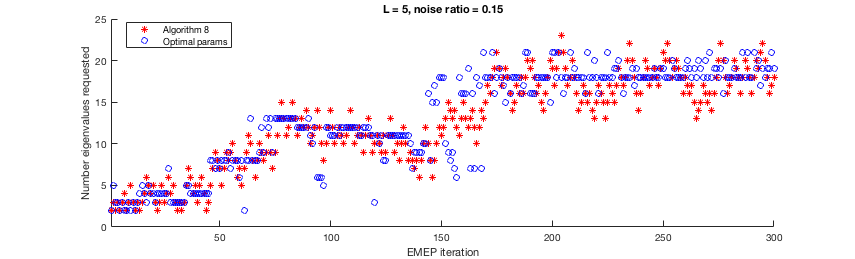
\includegraphics[scale=0.6]{Numerics-num_eigs_ada_vs_opt_1} }\vspace{0.6cm}
\vspace{0.2cm}
	\caption{
	Plot comparing Algorithm \ref{Alg:adaptive_IRAM} with the optimal choice of parameter $r$ (number of requested eigenvalues in the IRAM).
	 The \emep \ is from Figure \ref{Fig:Numerics-num_matvecs_orig_vs_optimal_params} and Arnoldi decomposition (\ref{Eqn:Arnoldi_decomp}) size is $m=40$.
	}
\label{Fig:Numerics-num_eigs_ada_vs_opt_one_plot}
\end{figure}
% experiments.figure.noisyimage_adaptive_eig_full_exp

Figure \ref{Fig:Numerics-num_eigs_ada_vs_opt_one_plot} shows that the parameter values $r_k$ chosen by Algorithm \ref{Alg:adaptive_IRAM} effectively track the optimal parameters for the IRAM.  
For the majority of iterates, the value $r_k$ is within two units from the optimal parameter value.
As we will see in Section \ref{Subsec:evol_mats-correl_btwn_EMEP_and_IRAM}, these changes in $r_k$ are related to the evolving spectrum of the \emep.




 


\section{Spectrum Distribution and IRAM Behavior}
\label{Subsec:evol_mats-correl_btwn_EMEP_and_IRAM}



In this section we examine an observed correlation between the clustering of the algebraically largest eigenvalues in the \emep \ and the convergence behavior of the IRAM (Algorithm \ref{Alg:IRAM}) for various parameters.
As we saw in Section \ref{Subsec:PLGD_term_crit-stagnation}, PLGD models with Gaussian noise (\ref{Eqn:PhaseLift-GD_Gaussian_noise}) typically have optimal EMEP matrices $\caA^*y_\star$ for which the algebraically largest eigenvalue has multiplicity greater than one.
Thus we may expect the algebraically largest eigenvalues in the EMEP to cluster for later iterates.

In Section \ref{Subsubsec:evol_mats-correl_clustering_IRAM_param} we examine two PLGD models and show that as the eigenvalues in the EMEP begin to cluster, the \textit{optimal} IRAM parameter $\bar{r}$ (i.e., the number of requested eigenvalues $r$ with the minimum number of matrix-vector products) increases such that $\lambda_{\bar{r}+1}$ is not clustered with $\lambda_1, \lambda_2, \ldots, \lambda_{\bar{r}}$.
We also see that the value $r_k$ chosen by Algorithm \ref{Alg:adaptive_IRAM} properly tracks the optimal parameter $\bar{r}_k$ for these two PLGD models.
Next, Section \ref{Subsubsec:evol_mats-default_Arnoldi_decomp_size} uses these two PLGD models to demonstrate that the Arnoldi decomposition (\ref{Eqn:Arnoldi_decomp}) size $m=40$ is sufficiently large for the IRAM to perform efficiently, and thus $m=40$ is an appropriate default parameter for Algorithm \ref{Alg:adaptive_IRAM}.





To illustrate these observations, we focus on the EMEP of two particular PLGD models with Gaussian noise (\ref{Eqn:PhaseLift-GD_Gaussian_noise}) for which the sequence of parameters $r_1, r_2, \ldots r_{maxit}$ chosen by Algorithm \ref{Alg:adaptive_IRAM} varies greatly.

\begin{figure}[H]
\centering
\hbox{\hspace{-1.8cm} 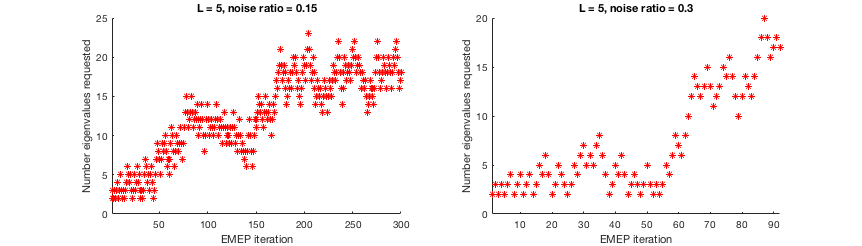
\includegraphics[scale=0.6]{Numerics-num_eigs_req_ada_2_exps} }\vspace{0.0cm}
	\caption{
Number of requested eigenvalues $r$ chosen by Algorithm \ref{Alg:adaptive_IRAM} for the \emep \ from two PLGD models with Gaussian noise (\ref{Eqn:PhaseLift-GD_Gaussian_noise}), with noise ratio $\epsilon_\text{rel}=0.15, 0.30$, oversampling rate $L=5$, and original signal from Figure \ref{Fig:parrot_signal_iterates} resized to $64 \times 64$ pixels.
}
\label{Fig:Numerics-num_req_eigs_2_exps}
\end{figure}
% experiments.figure.noisyimage_adaptive_eig_full_exp



For both PLGD models in Figure \ref{Fig:Numerics-num_req_eigs_2_exps}, changes in the EMEP caused Algorithm \ref{Alg:adaptive_IRAM} to increase the number of requested eigenvalues $r_k$ significantly from early to later iterates $k$.
Yet the value of $r_k$ increased at a quicker rate for the experiment in Figure \ref{Fig:Numerics-num_req_eigs_2_exps} with $L=5$ and $\epsilon_\text{rel} = 0.30$.
As we will see in Section \ref{Subsubsec:evol_mats-correl_clustering_IRAM_param}, this quick increase from $r_{55}=3$ to $r_{70}=13$ coincides with a sudden clustering of the algebraically largest eigenvalues in the EMEP.





\subsection{Eigenvalue Clustering and IRAM Parameter Choice}		\label{Subsubsec:evol_mats-correl_clustering_IRAM_param}




We now show that the PLGD models in Figure \ref{Fig:Numerics-num_req_eigs_2_exps} exhibit a correlation between the spectrum distribution of the \emep \ and the convergence behavior of the IRAM (Algorithm \ref{Alg:IRAM}).
For these two models, as the algebraically largest eigenvalues $\lambda_1, \lambda_2, \ldots, \lambda_{m-1}, \lambda_{m}$ of the EMEP begin to cluster, 
the IRAM converges much faster if the number of requested eigenvalues $r<m$ is large enough such that $\lambda_{r+1}$ is not clustered with $\lambda_1, \lambda_2, \ldots, \lambda_r$.
Thus, as Algorithm \ref{Alg:adaptive_IRAM} explicitly tracks the optimal sequence of parameters $\bar{r}_k$, this algorithm implicitly tracks the clustering of the algebraically largest eigenvalues in the EMEP.
To demonstrate these observations, we consider various EMEP iterates $k$ and number of requested eigenvalues $r$, and plot the numbers of matrix-vector products for the IRAM as well as the eigenvalue difference $\lambda_{r+1} - \lambda_r$.
Figures \ref{Fig:Numerics-surf_mvs_eig_diffs_1} and \ref{Fig:Numerics-surf_mvs_eig_diffs_2} depict about half of the EMEP iterates from the two PLGD models in Figure \ref{Fig:Numerics-num_req_eigs_2_exps}, so we may focus on the regions where $r_k$ in Algorithm \ref{Alg:adaptive_IRAM} varies greatest.





\begin{figure}[H]
\centering
\hbox{\hspace{-0.5cm} 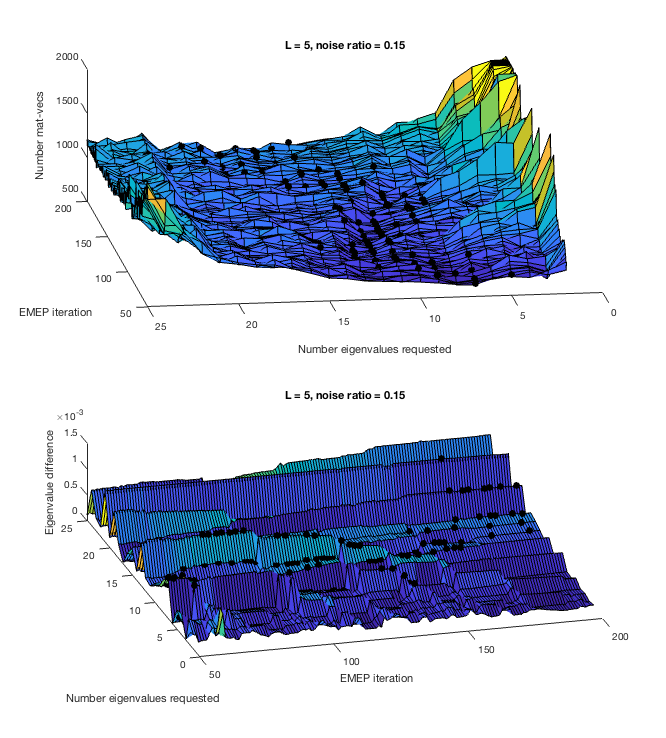
\includegraphics[scale=0.65]{Numerics-surf_num_mvs_and_eig_diffs_1} }\vspace{0.0cm}
	\caption{Behavior of Algorithm \ref{Alg:adaptive_IRAM} for the experiment from Figure \ref{Fig:Numerics-num_req_eigs_2_exps} with $L=5$, $\epsilon_\text{rel}=0.15$.  Top: Number of matrix-vector products (capped at 2,000 for better viewing) for each \emep \ iterate $k$ and number of requested eigenvalues $r$. Bottom: eigenvalue differences $\lambda_r - \lambda_{r+1}$ for each \emep \ iterate $k$ and number of requested eigenvalues $r$.  Black dots in both plots indicate the value $r_k$ chosen by Algorithm \ref{Alg:adaptive_IRAM}.}
\label{Fig:Numerics-surf_mvs_eig_diffs_1}
\end{figure}
% experiments.figure.noisyimage_adaptive_eig_full_exp



\begin{figure}[H]
\centering
\hbox{\hspace{-0.5cm} 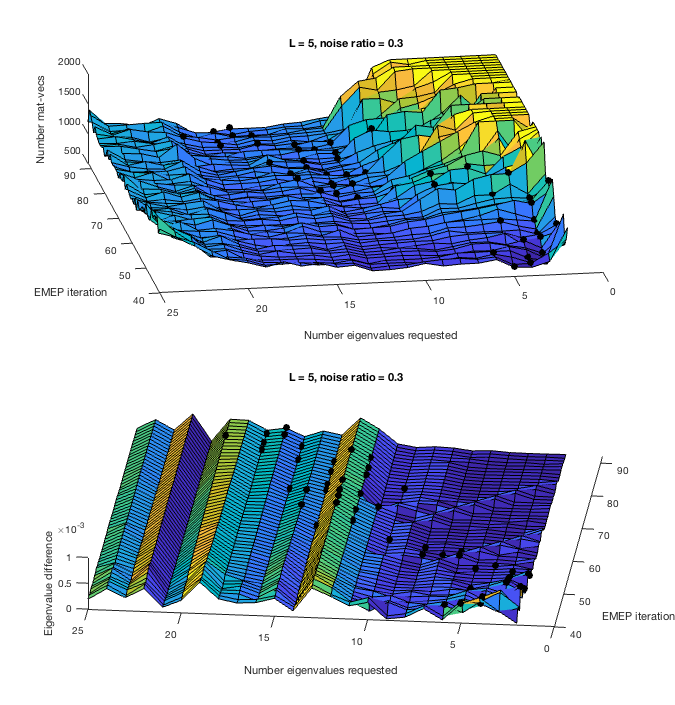
\includegraphics[scale=0.65]{Numerics-surf_num_mvs_and_eig_diffs_2} }\vspace{0.0cm}
	\caption{Behavior of Algorithm \ref{Alg:adaptive_IRAM} for the experiment from Figure \ref{Fig:Numerics-num_req_eigs_2_exps} with $L=5$, $\epsilon_\text{rel}=0.30$.  Top: Number of matrix-vector products (capped at 2,000 for better viewing) for each \emep \ iterate $k$ and number of requested eigenvalues $r$. Bottom: eigenvalue differences $\lambda_r - \lambda_{r+1}$ for each \emep \ iterate $k$ and number of requested eigenvalues $r$.  Black dots in both plots indicate the value $r_k$ chosen by Algorithm \ref{Alg:adaptive_IRAM}.}
\label{Fig:Numerics-surf_mvs_eig_diffs_2}
\end{figure}
% experiments.figure.noisyimage_adaptive_eig_full_exp





In Figures \ref{Fig:Numerics-surf_mvs_eig_diffs_1} and \ref{Fig:Numerics-surf_mvs_eig_diffs_2} we see that the clustering of the algebraically largest eigenvalues corresponds to an increase in the optimal number of requested eigenvalues $\bar{r}_k$ for later \emep \ iterates $k$.
In Figure \ref{Fig:Numerics-surf_mvs_eig_diffs_1}, the eigenvalues $\lambda_1, \lambda_2, \ldots, \lambda_{10}$ cluster around iterates $125 \leq k \leq 175$; and likewise the optimal parameter $\bar{r}_{125} \approx 10$ increases to $\bar{r}_{175} \approx 18$.
Figure \ref{Fig:Numerics-surf_mvs_eig_diffs_2} depicts a similar shift, where the eigenvalues $\lambda_1, \lambda_2, \ldots, \lambda_{10}$ cluster around iterates $50 \leq k \leq 70$, and the optimal parameter increases to $\bar{r}_{70} \approx 15$.
In the case of Figure \ref{Fig:Numerics-surf_mvs_eig_diffs_2}, the most tightly clustered eigenvalues $\lambda_1, \lambda_2, \ldots, \lambda_{8}$ also correspond to parameter values $r = 2, 3, \ldots, 7$ for which the IRAM required the greatest number of matrix-vector products to converge.



This observed correlation between eigenvalue clustering and a change in the convergence rate of the IRAM may be related to the subroutines used in the IRAM.
As discussed in Section \ref{Subsec:evol_mats-IRAM}, the IRAM is based on the following two algorithms.
Given a Hermitian matrix $A \in \bbC^{n \times n}$, the $m$-step Arnoldi iteration (Algorithm \ref{Alg:Arnoldi_iteration}) generates a set of Ritz pairs $(\theta_1, u_1), (\theta_2, u_2), \ldots, (\theta_m, u_m)$ for $A$ with respect to $\caK_m(A, q_1)$.
Next, the $p$-step shifted QR iteration (Algorithm \ref{Alg:shifted_QR_iteration}) restarts the Arnoldi decomposition (\ref{Eqn:Arnoldi_decomp}) by attempting to damp the unwanted part of the spectrum using the Ritz values $\{ \theta_{r+1}, \theta_{r+2}, \ldots, \theta_m \}$ (where $m = r + p$).
Assume we have an EMEP matrix iterate $A_k$ with some number $s$ of clustered algebraically largest eigenvalues, $\lambda_1 \approx \lambda_2 \approx \cdots \approx \lambda_s$; 
and assume we select the number of requested eigenvalues $r < s$.
When the IRAM builds an Arnoldi decomposition (\ref{Eqn:Arnoldi_decomp}), the $s$ largest Ritz values of $A_k$ with respect to $\caK_m(A_k, q_1)$ may include values $\theta_{r+1}, \theta_{r+2}, \ldots, \theta_s$ which are close approximations to the desired eigenvalues.
Thus when the shift values $\mu_1 = \theta_{r+1}, \mu_2 = \theta_{r+2}, \ldots, \mu_{s-r} = \theta_{s}, \ldots, \mu_p = \theta_m$ are passed to the $p$-step shifted QR iteration, the implicit polynomial filter (\ref{Eqn:filter_poly}) will include values $\mu_1, \mu_2, \ldots, \mu_{s-r}$ which damp the desired part of the spectrum.
Thus, if $r < s$ we may expect the IRAM to converge more slowly.
However, if we select the number of requested eigenvalues $r > s$, then the shift values used in the $p$-step shifted QR iteration will always include parts of the spectrum which we want to damp and we may expect the IRAM to converge more quickly. 


Figures \ref{Fig:Numerics-surf_mvs_eig_diffs_1} and \ref{Fig:Numerics-surf_mvs_eig_diffs_2} also demonstrate that Algorithm \ref{Alg:adaptive_IRAM} properly tracks the optimal number of requested eigenvalues $\bar{r}_k$ as this value changes.
In particular, Figure \ref{Fig:Numerics-surf_mvs_eig_diffs_2} indicates that $\bar{r}_k$ increased quickly from iterates $k = 50$ to $k = 70$.
Likewise, Algorithm \ref{Alg:adaptive_IRAM} increased $r_k$ by two units for several iterates $55 \leq k \leq 70$ (see Figure \ref{Fig:Numerics-num_req_eigs_2_exps}).
These two-unit increases were the result of Algorithm \ref{Alg:adaptive_IRAM} properly identifying a quick increase in the number of matrix-vector products $t_k$ for smaller values $r_k$.
Recall that Algorithm \ref{Alg:adaptive_IRAM} determines the update $r_{k+1}$ using two-point and four-point linear interpolations (equations (\ref{Eqn:adaptive_delta_2}) and (\ref{Eqn:adaptive_delta_4_lin_interp_prob}), respectively) of the previous parameters $r_k$ and $t_k$.
For the PLGD model in Figure \ref{Fig:Numerics-surf_mvs_eig_diffs_2}, both of these interpolations agreed (i.e., $\delta_2=1$ in (\ref{Eqn:adaptive_delta_2}) was equal to $\delta_4=1$ in (\ref{Eqn:adaptive_delta_4})) for several iterates $55 \leq k \leq 70$.
Thus Algorithm \ref{Alg:adaptive_IRAM} quickly increased $r_k$, avoiding excessive matrix-vector multiplications.







\subsection{Selecting the Arnoldi Decomposition Size}		\label{Subsubsec:evol_mats-default_Arnoldi_decomp_size}



Next we show that the default parameter setting $m = 40$ in Algorithm \ref{Alg:adaptive_IRAM} is sufficiently large to minimize the number of matrix-vector products in the EMEP in the models from Figure \ref{Fig:Numerics-num_req_eigs_2_exps}.
To demonstrate that $m=40$ is appropriate, we will examine a more difficult eigenvalue problem (i.e., later iterate) from each of these models.
Figure \ref{Fig:Numerics-surf_mvs_for_m_vs_j} depicts the number of matrix-vector products for various IRAM parameters $r$ and $m$ for an iterate from each model.


\begin{figure}[H]
\centering
\hbox{\hspace{-0.1cm} 
	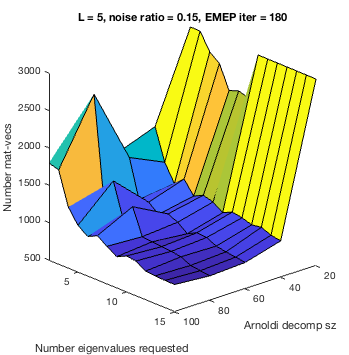
\includegraphics[scale=0.6]{Numerics-surf_mvs_for_m_vs_j_1}
	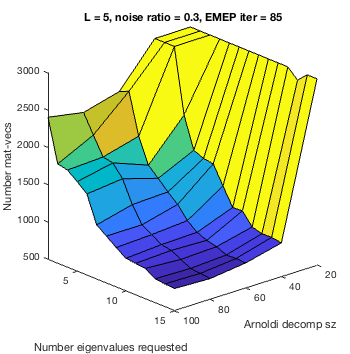
\includegraphics[scale=0.6]{Numerics-surf_mvs_for_m_vs_j_2} 
			}
	\vspace{0.0cm}
	\caption{
Number of matrix-vector products (capped at 3,000 for better viewing) for individual \emep \ iterates with varying number of requested eigenvalues $r$ and Arnoldi decomposition (\ref{Eqn:Arnoldi_decomp}) size $m$.  
Left: EMEP iterate 180 from Figure \ref{Fig:Numerics-surf_mvs_eig_diffs_1}.
Right: EMEP iterate 85 from Figure \ref{Fig:Numerics-surf_mvs_eig_diffs_2}.
	}
\label{Fig:Numerics-surf_mvs_for_m_vs_j}
\end{figure}
% experiments.figure.noisyimage_adaptive_eig_full_exp




Figure \ref{Fig:Numerics-surf_mvs_for_m_vs_j} suggests that we should not select IRAM parameters below $r = 9$ and $m = 40$ for the EMEP iterate in the left plot, nor should we select parameters below $r = 12$ and $m = 40$ for the EMEP iterate in the right plot.  
Yet there is no significant benefit to selecting larger parameter values.
Since the EMEP iterates in Figure \ref{Fig:Numerics-surf_mvs_for_m_vs_j} represent later, more difficult eigenvalue problems, this figure suggests that $m = 40$ is sufficiently large for all iterates.
Thus we select a fixed Arnoldi decomposition (\ref{Eqn:Arnoldi_decomp}) size $m = 40$ for Algorithm \ref{Alg:adaptive_IRAM}.






